\documentclass[a4paper]{article}

\usepackage[T1]{fontenc}
\usepackage[utf8]{inputenc}

\usepackage{mathptmx}

\usepackage{subcaption}
\usepackage[shortlabels]{enumitem}
\usepackage{amsmath,amssymb}
\usepackage{amsthm}
\usepackage{bbm}
\usepackage{graphicx}
\usepackage[colorlinks=true,naturalnames=true,plainpages=false,pdfpagelabels=true]{hyperref}
\usepackage[parfill]{parskip}

\usepackage{tikz}
\usetikzlibrary{patterns,decorations.pathmorphing,positioning}

\usepackage[framemethod=TikZ]{mdframed}

\tikzstyle{titlered} =
    [draw=black, thick, fill=white,%
        text=black, rectangle,
        right, minimum height=.7cm]

\newcounter{exercise}

\renewcommand*\theexercise{Exercise~\arabic{exercise}}

\makeatletter
\mdfdefinestyle{exercisestyle}{%
    outerlinewidth=1em,%
    outerlinecolor=white,%
    leftmargin=-1em,%
    rightmargin=-1em,%
    middlelinewidth=1.2pt,%
    roundcorner=5pt,%
    linecolor=black,%
    backgroundcolor=blue!5,
    innertopmargin=1.2\baselineskip,
    skipabove={\dimexpr0.5\baselineskip+\topskip\relax},
    skipbelow={-1em},
    needspace=3\baselineskip,
    frametitlefont=\sffamily\bfseries,
    settings={\global\stepcounter{exercise}},
    singleextra={%
        \node[titlered,xshift=1cm] at (P-|O) %
            {~\mdf@frametitlefont{\theexercise}~};},%
    firstextra={%
            \node[titlered,xshift=1cm] at (P-|O) %
                    {~\mdf@frametitlefont{\theexercise}~};},
}
\makeatother

\newenvironment{MyExercise}%
{\begin{mdframed}[style=exercisestyle]}{\end{mdframed}}

\theoremstyle{definition}
\newtheorem{definition}{Definition}

\theoremstyle{definition}
\newtheorem{question}{Question}

\theoremstyle{definition}
\newtheorem{example}{Example}

\theoremstyle{theorem}
\newtheorem{theorem}{Theorem}

\theoremstyle{theorem}
\newtheorem{lemma}{Lemma}

\newtheorem*{idea}{Proof Idea}



\title{University of Vienna\\ Faculty of Physics\\ \vspace{1.25cm}
Notes on\\ Noncommutative Geometry and Particle Phyiscs}
\author{Milutin Popovic \\ Supervisor: Dr. Lisa
Glaser}
\date{Week 5: 12.03 - 19.03}

\begin{document}

    \maketitle
    \tableofcontents
    \newpage

\section{Noncommutative Geometric Spaces }
\subsection{Exercises}

\begin{MyExercise}
\textbf{
    Make the proof of the last theorem (see week4.pdf) explicit for $N=3$.
}\newline

    For the C* algebra we have $A=\mathbb{C}^3$
    For $H$ we have $H = (\mathbb{C}^2)^{\oplus 3} = H_2 \oplus H_2^1 \oplus H_2^2$.
    The symmetric operator $D$ acting on $H$ and the representation $\pi (a)$:
    \begin{align}
        \pi((a(1), a(2), a(3)) &=
        \begin{pmatrix}
            a(1) & 0 \\ 0 & a(2)
        \end{pmatrix} \oplus
        \begin{pmatrix}
            a(1) & 0 \\ 0 & a(3)
        \end{pmatrix} \oplus
        \begin{pmatrix}
            a(2) & 0 \\ 0 & a(2)
        \end{pmatrix} \nonumber  \\
        & =
        \begin{pmatrix}
            a(1) & 0 & 0 & 0 & 0 & 0 \\
            0    & a(2) & 0 & 0 & 0 & 0 \\
            0    & 0 & a(1) & 0 & 0 & 0 \\
            0    & 0 & 0 & a(3) & 0 & 0 \\
            0    & 0 & 0 & 0 & a(2) & 0 \\
            0    & 0 & 0 & 0 & 0 & a(3)
        \end{pmatrix} \\
        D &=
        \begin{pmatrix}
            0 & x_1 \\ x_1 & 0
        \end{pmatrix} \oplus
        \begin{pmatrix}
            0 & x_2 \\ x_2 & 0
        \end{pmatrix} \oplus
        \begin{pmatrix}
            0 & x_3 \\ x_3 & 0
        \end{pmatrix} \nonumber \\
        &=
        \begin{pmatrix}
            0   & x_1 & 0 & 0 & 0 & 0 \\
            x_1 & 0   & 0 & 0 & 0 & 0 \\
            0   & 0   & 0 & x_2 & 0 & 0 \\
            0   & 0   & x_2 & 0 & 0 & 0 \\
            0   & 0   & 0 & 0 & 0 & x_3 \\
            0   & 0   & 0 & 0 & x_3 & 0 \\
        \end{pmatrix} \\
    \end{align}
    Then the norm of the commutator would be the largest eigenvalue
    \begin{align}
        &||[D, \pi(a)]|| = ||D\pi(a) - \pi(a)D||\nonumber\\
        &=
        \left|\left|
    \setlength{\arraycolsep}{0.1cm}
      \renewcommand{\arraystretch}{0.1}
        \begin{pmatrix}
            0   & x_1(a(2)-a(1)) & 0 & 0 & 0 & 0 \\
            -x_1(a(2)-a(1)) & 0   & 0 & 0 & 0 & 0 \\
            0   & 0   & 0 & x_2(a(3)-a(1)) & 0 & 0 \\
            0   & 0   & -x_2(a(3)-a(1)) & 0 & 0 & 0 \\
            0   & 0   & 0 & 0 & 0 & x_3(a(3)-a(2)) \\
            0   & 0   & 0 & 0 & -x_3(a(2)-a(3)) & 0 \\
        \end{pmatrix}\right|\right| \label{skew matrix}
    \end{align}
The matrix in Equation \ref{shew matrix} is a skew symmetric matrix its eigenvalues
are $i\lambda_1, i\lambda_2, i\lambda_3, i\lambda_4$, where the $\lambda$'s are on the
upper and lower diagonal check \url{https://en.wikipedia.org/wiki/Skew-symmetric_
matrix#Skew-symmetrizable_matrix}. The matrix norm of would be the maximum of the norm of
the larges eigenvalues:
\begin{align}
    ||[D, \pi(a)]|| = \max_{a\in A}\{&x_1|a(2)-a(1)|,\\
    &x_2|(a(3)-a(1))|,\nonumber\\
    &x_3|(a(3)-a(2))|,\}\nonumber
\end{align}
The metric is then:
\begin{align}
    d =
    \begin{pmatrix}
        0 & a(1)-a(2) & a(1)-a(3)\\
        a(2)-a(1) & 0 & a(2)-a(3)\\
        a(3)-a(1) & a(3)-a(2) & 0
    \end{pmatrix}
\end{align}
\end{MyExercise}

\begin{MyExercise}
    \textbf{
	Compute the metric on the space of three points given by $d_{ij} =
	\sup_{a\in A}\{|a(i) - a(j)|: ||[D, \pi(a)]|| \leq 1\}$ for the set of data
    $A = \mathbb{C}^3$ acting in the defining representation $H = \mathbb{C}^3$, and
    \begin{align}
    D =
    \begin{pmatrix}
        0 & d^{-1} & 0 \\
        d^{-1} & 0 & 0 \\
        0 & 0 & 0
    \end{pmatrix}
    \end{align}
    for some $d \in \mathbb{R}$
}\newline

    We have $A=\mathbb{C}^3$, $H=\mathbb{C}^3$ and $D$ from above, then

    \begin{align}
        ||[D, \pi(a)]|| &= d^{-1}\left|\left|
    \begin{pmatrix}
        0 & a(2)-a(1) & 0 \\
        -(a(2)-a(1)) & 0 & 0 \\
        0 & 0 & 0
    \end{pmatrix} \right|\right|
    \end{align}
    The metric is then
    \begin{align}
    d =
        \begin{pmatrix}
            0 & a(1)-a(2) & a(1)  \\
            a(2)-a(1) & 0 & a(2) \\
            -a(1) & -a(2) & 0
        \end{pmatrix}
    \end{align}
\end{MyExercise}

\begin{MyExercise}
    \textbf{
    Show that $d_{ij}$ from Equation \ref{ext metric} is a metric on $\hat{A}$ by
    establishing that:
    \begin{align}
        d_{ij} &= 0\;\;\; \Leftrightarrow \;\;\; i=j \label{metric 1} \\
        d_{ij} &= d_{ji} \label{metric 2}\\
        d_{ij} &\leq d_{ik} + d_{kj} \label{metric 3}
    \end{align}
    \begin{equation} \label{ext metric}
        d_{ij} = \sup_{a\in A}\big\{|\text{Tr}(a(i)) - \text{Tr}((a(j))|: ||[D, a]|| \leq 1\big\}
    \end{equation}
}\newline

For Equation \ref{metric 1} set $i=j$ in \ref{ext metric}.
\begin{align}
    d_{ii} &= \sup_{a \in A}\{|\text{Tr}(a(i)) - \text{Tr}((a(i))|: ||[D, a]|| \leq
    1\big\} \\
    &= \sup_{a \in A}\{0: ||[D, a]|| \leq 1\big\} = 0
\end{align}
For Equation \ref{metric 2} obviously we have the commuting property of
addition.
\newline
For Equation \ref{metric 3}, for $k=j$ then $d_{kj} = 0$ and the equality
holds. For $i = k$ then $d_{ik} = 0$ and equality holds. Else set $d_{ik} =
1$ and $d_{kj} = 1$ then $d_{ij} = 1 \leq d_{ik} + d_{kj} = 2$
\end{MyExercise}

\subsection{Properties of Matrix Algebras}
\begin{lemma}
    If $A$ is a unital C* algebra that acts faithfully on a finite
    dimensional Hilbert space, then $A$ is a matrix algebra of the Form:
    \begin{equation}
        A \simeq \bigoplus _{i=1}^N M_{n_i}(\mathbb{C})
    \end{equation}
\end{lemma}
\begin{proof}
    Since $A$ acts faithfully on a Hilbert space, then $A$ is a C*
    subalgebra of a matrix algebra $L(H) = M_{\dim (H)}(\mathbb{C}
    \Rightarrow A \simeq \text{Matrix algebra}$.
\end{proof}

\begin{question}
    What does the author mean when he sais 'acts faithfully on a
    Hilbertspace`? Then the representation is fully reducible, or that the
    presentation is irreducible?
    \newline

    For a *-representation 'faithful` if it is injective. For a
    *-homomorphism 'faithful` means one-to-one correspondance
\end{question}

\begin{example}
    $A = M_n(\mathbb{C})$ and $H=\mathbb{C}^n$, $A$ acts on $H$ with matrix
    multiplication and standard inner product. $D$ on $H$ is a hermitian
    matrix $n\times n$ matrix.
\end{example}

$D$ is referred to as a finite Dirac operator as in as its $\infty$
dimensional on Riemannian Spin manifolds coming in Chapter 4.
\newline

Now can introduce a 'differential 'geometric structure` on the finite space X
with the \textbf{devided difference}
\begin{equation}
    \frac{a(i)-a(j)}{d_{ij}}
\end{equation}
for each pair $i$, $j$ $\in X$ the finite dimensional discrete space $X$.
This appears in the entries in the commutator $[D, a]$ in the above
exercises.

\begin{definition}
    Given an finite spectral triple $(A, H, D)$, the $A$-bimodule of
    Connes' differential one-forms is:
    \begin{equation}
        \Omega _D ^1 (A) := \left\{ \sum _k a_k[D, b_k]: a_k, b_k \in A \right\}
    \end{equation}
\end{definition}

\begin{question}
    Is the Conne's differential one form  the set of all '1st order
    differential operators` given $A$, that act on $H$?
\end{question}
Then there is a map $d:A\rightarrow \Omega _D ^1 (A)$, $d = [D, \cdot]$.
\begin{MyExercise}
    \textbf{
    Verify that 'd` is a derivation of the C* algebra
    \begin{align}
        d(ab) = d(a)b + ad(b) \\
        d(a^*) = -d(a)^*
    \end{align}
}\newline

    For the record $d(\cdot) = [D, \cdot]$, then we have
    \begin{enumerate}
        \item
            \begin{align}
                d(ab) &= [D, ab] = [D, a]b + a[D,b]\\
                &= d(a)b + ad(b)
            \end{align}
        \item
            \begin{align}
                d(a^*) &= [D, a^*] = Da^* - a^*D \\
                &=-(D^*a - aD^*) = -[D^*, a] \\
                &= -d(a)^*
            \end{align}
    \end{enumerate}
\end{MyExercise}
\begin{MyExercise}
    \textbf{
    Verify that $\Omega _D^1 (A)$ is an $A$-bimodule by rewriting
    }
    \begin{align}
        a(a_k[D, b_k])b = \sum_k a'_k[D, b'_k] \;\;\;\; a'_k, b'_k \in A
    \end{align}
    \newline

    Begin
    \begin{align}
        a(a_k[D, b_k])b &= aa_k(Db_k - b_k D) b = \\
           &= aa_k(Db_k b - b_k D b) = aa_k(Db_k b - b_k Db - b_kbD +b_kbD)=\\
           &= aa_k(Db_kb-b_kbD + b_k b D - b_k D b) = \\
           &= aa_k [D, b_kb] + aa_k b [D, b]=\\
           &= \sum _k a_k' [D, b_k']
    \end{align}

\end{MyExercise}

\begin{lemma}
    Let $(A, H, D) = (M_n(\mathbb{C}, \mathbb{C}^n, D)$, with $D$ a hermitian
    $n\times n$ matrix. If $D$ is not a multiple of the identity then:
    \begin{equation}
        \Omega _D ^1 (A)  \simeq  M_n(\mathbb{C}) = A
    \end{equation}
\end{lemma}

\begin{proof}
    Assume $D = \sum _i \lambda _i e_{ii}$ (diagonal), $\lambda _i \in \mathbb{R}$ and
    $\{e_{ij}\}$ the basis of $M_n(\mathbb{C}$. For fixed $i$, $j$ choose $k$
    such that $\lambda _k \neq \lambda _j$ then
    \begin{align} \label{basis}
        \left(\frac{1}{\lambda _k - \lambda _j} e_{ik}\right) [D, e_{kj}] =
        e_{ij}
    \end{align}
    $e_{ij}\in \Omega _D ^1 (A)$ by the above definition. And $\Omega _D ^1
    (A) \subset L(\mathbb{C}^n) = H \simeq M_n(\mathbb{C}) = A$
\end{proof}

\begin{MyExercise}
    \textbf{
     Consider $(A=\mathbb{C}^2, H=\mathbb{C}^2,
     D = \begin{pmatrix} 0 & \lambda \\ \bar{\lambda} & 0
     \end{pmatrix})$ with $\lambda \neq 0$. Show that $\Omega _D^1(A)
     \simeq M_2(\mathbb{C})$
 }
\newline

    Because of the Hilbert Basis $D$ can be extended in terms of
    the basis of $M_2(\mathbb{C})$, plugging this into Equation
    \ref{basis} will get us the same cyclic result, thus
    $\Omega _D^1(A) \simeq M_2(\mathbb{C})$
\
\end{MyExercise}

\subsection{Morphisms Between Finite Spectral Triples}
\begin{definition}
    two finite spectral tripes $(A_1, H_1, D_1)$ and $(A_2, H_2, D_2)$ are
    called unitarily equivalent if
    \begin{itemize}
        \item $A_1 = A_2$
        \item $\exists \;\; U: H_1 \rightarrow H_2$, unitary with
            \begin{enumerate}
                \item  $U\pi_1(a)U^* = \pi_2(a)$ with $a \in A_1$
                \item  $UD_1 U^* = D_2$
            \end{enumerate}
    \end{itemize}
\end{definition}

Some remarks
\begin{itemize}
    \item the above is an equivalence relation
    \item spectral unitary equivalence is given by the unitaries of the
        matrix algebra itself
    \item for any such $U$ then $(A, H, D) \sim (A, H, UDU^*)$
    \item $UDU^* = D + U[D, U^*]$ of the form of elements in
        $\Omega _D^1 (A)$.
\end{itemize}

\begin{MyExercise}
    \textbf{
    Show that the unitary equivalence between finite spectral
    triples is a equivalence relation
}\newline

    An equivalence relation needs to satisfy reflexivity, symmetry
    transitivity.
    Let $(A_1, H_1, D_1)$, $(A_2, H_2, D_2)$ and $(A_3, H_3, D_3)$
    be three finite spectral triples.
    \newline

    For reflexivity $(A_1, H_1, D_1) \sim (A_1, H_1, D_1)$. So there
    exists a $U: H_1 \rightarrow H_1$ unitary, which is the identity
    and always exists.
    \newline

    For symmetry we need
    \begin{align}
        (A_1, H_1, D_1) \sim (A_2, H_2, D_2) \Leftrightarrow
        (A_2, H_2, D_2) \sim (A_1, H_1, D_1)
    \end{align}
    because $U$ is unitary:
    \begin{align}
        &U\pi_1(a)U^* = \pi_2(a) \;\;\; | \cdot U^*\boxdot U \\
        &U^*U\pi_1(a)U^*U = \pi_1(a) = U^*\pi_2(a)U \\
    \end{align}
    The same with the symmetric operator $D$.
    \newline

    For transitivity we need
    \begin{align}
        (A_1, H_1, D_1) &\sim (A_2, H_2, D_2) \;\;\; \text{and} \;\;\;
        (A_2, H_2, D_2) \sim (A_3, H_3, D_3) \\
        &\Rightarrow (A_1, H_1, D_1) \sim (A_3, H_3, D_3)
    \end{align}
    There are two unitary maps $U_{12}:H_1 \rightarrow H_2$ and
    $U_{23}: H_2 \rightarrow H_3$ then
    \begin{align}
        U_{23}U_{12} \pi_1(a) U^*_{12}U^*_{23} &= U_{23}
        \pi_2(a) U_23^* \\
        &= \pi_3(a) \\
        U_{23}U_{12} D_1U^*_{12}U^*_{23} &= U_{23}
        D_2 U_23^* \\
        &= D_3
    \end{align}
\end{MyExercise}

Extending the this relation we look again at  the notion of equivalence from
Morita equivalence of Matrix Algebras.
\newline

\begin{definition}
    Let $A$ be an algebra. We say that $I \subset A$, as a vector space, is a
    right(left) ideal if $ab \in I$ for $a \in A$ and $b\in I$ (or $ba \in
    I$, $b\in I$, $a\in A$). We call a left-right ideal simply an ideal.
\end{definition}

Given a Hilbert bimodule $E \in KK_f(B, A)$ and $(A, H, D)$ we construct
a finite spectral triple on $B$, $(B, H', D')$
\begin{equation}
    H' = E \otimes _A H
\end{equation}
We might define $D'$ with $D'(e \otimes \xi) = e\otimes D\xi$, thought this
would not satisfy the ideal defining the balanced tensor product over $A$,
which is generated by elements of the form
\begin{align}
    e a \otimes \xi - e\otimes a \xi ;\;\;\;\; e\in E, a\in A, \xi \in H
\end{align}
This inherits the left action on $B$ from $E$ and has a $\mathbb{C}$
valued inner product space. $B$ also satisfies the ideal.
\begin{equation}
    D'(e\otimes \xi) = e \otimes D \xi + \nabla (e) \xi \;\;\;\; e\in
    E, a\in A
\end{equation}
Where $\nabla$ is called the \textit{connection on the right A-module E}
associated with the  derivation $d=[D, \cdot]$ and satisfying the
\textit{Leibnitz Rule} which is
\begin{equation}
    \nabla(ae) = \nabla(e)a + e \otimes [D, a] \;\;\;\;\;  e\in E,\; a\in A
\end{equation}
Then $D'$ is well defined on $E \otimes _A H$:
\begin{align}
    D'(ea \otimes \xi - e \otimes a \xi) &=  D'(ea \otimes \xi) - D'(e
    \otimes \xi) \\
    &= ea\otimes D\xi + \nabla(ae) \xi - e \otimes D(a\xi ) - \nabla (e)a
    \xi \\
    &= 0.
\end{align}
With the information thus far we can prove the following theorem
\begin{theorem}
    If $(A, H, D)$ a finite spectral triple, $E \in KK_f(B, A)$.
    Then $(V, E\otimes _A H, D')$ is a finite spectral triple, provided that
    $\nabla$ satisfies the compatibility condition
    \begin{equation}
        \langle e_1, \nabla e_2 \rangle _E - \langle \nabla e_1, e_2
        \rangle _E = d\langle e_1, e_2 \rangle _E \;\;\;\; e_1, e_2 \in E
    \end{equation}
\end{theorem}
\begin{proof}
    $E\otimes _A H$ was shown in the previous section (text before the
    theorem). The only thing left is to show that $D'$ is a symmetric
    operator, this we can just compute. Let $e_1, e_2 \in E$ and $\xi _1,
    \xi _2 \in H$ then
    \begin{align}
        \langle e_1 \otimes \xi _1, D'(e_2 \otimes \xi_2)\rangle _{E\otimes _A H} &=
        \langle \xi _1, \langle e_1, \nabla e_2\rangle _E  \xi _2\rangle  + \langle \xi _1 , \langle e_1, e_2\rangle _E D\xi
        _2\rangle _H \\
        &= \langle \xi _1, \langle \nabla e_1, e_2\rangle _E \xi _2\rangle _H + \langle \xi _1, d\langle e_1, e_2\rangle  _E
        \xi _2\rangle _H \\
        &+ \langle D\xi _1,\langle e_1, e_2\rangle _E \xi _2\rangle _H - \langle \xi _1, [D, \langle e_1, e_2\rangle _E] \xi
        _2 \rangle _H \\
        &= \langle D'(e_1 \otimes \xi _1), e_2 \otimes \xi _2\rangle _{E \otimes _A H}
    \end{align}
\end{proof}

\begin{MyExercise}
    \textbf{
    Let $\nabla$ and $\nabla'$ be two connections on a right $A$-module
    $E$. Show that $\nabla - \nabla'$ is a right $A$-linear map
    $E \rightarrow E\otimes _A \Omega _D^1(A)$
}\newline

    Both $\nabla$ and $\nabla'$ need to satisfy the Leiblitz rule, so
    let's see if $\nabla - \nabla'$ does.

    \begin{align}
        \nabla(ea)-\nabla'(ea)&=\nabla(e) + e\otimes[D, a]\\
        &-(\nabla'(e)a + e\otimes[D',a])\\
        &=\bar{\nabla}a + e\otimes(Da-aD-D'a+aD')\\
        &=\bar{\nabla}a + e\otimes((D-D')a-a(D-D'))\\
        &=\bar{\nabla}a + e\otimes[D', a]\\
        &=\bar{\nabla}(ea)
    \end{align}
    Therefore $\nabla-\nabla'$ is a linear map.
\end{MyExercise}

\begin{MyExercise}
    \textbf{
    Construct a finite spectral triple $(A, H', D')$ from $(A, H, D)$
    \begin{enumerate}
        \item show that the derivation $d(\cdot):A \rightarrow A\otimes _A
            \Omega_D^1(A)=\Omega_D^1(A)$ is a connection on $A$
            considered a right $A$-module
        \item Upon identifying $A\otimes_A H\simeq H$, what is $D'$
            when the connection is $d(\cdot)$.
        \item Use 1) and 2) to show that any connection $\nabla:
            A\rightarrow A\otimes_A \Omega_D^1(A)$ is given by
            \begin{align}
                \nabla = d + \omega
            \end{align}
            where $\omega \in \Omega_D^1(A)$
        \item Upon identifying $A\otimes_A H \simeq H$, what is the
            difference operator $D'$ with the connection on $A$ given by
            $\nabla = d + \omega$
    \end{enumerate}
}
    \begin{enumerate}
        \item $\nabla(e \cdot a) =  d(a)$
        \item
            $D'(a\xi) = a(D\xi) + (\nabla a) \xi = D(a\xi)$
        \item Use the identity element $e \in A$\\
                $\nabla (e\cdot a) = \nabla(e) a + 1 \otimes d(a)=d(a)
                \nabla(e) a$
            \item $D'(a\otimes \xi) = D'(a \xi) = a(D\xi) + (\nabla a)\xi =
                a(D\xi) + \nabla(e \cdot a) \xi \\
                = D(a\xi) + \nabla(e) (a\xi)$
    \end{enumerate}
\end{MyExercise}

\subsection{Graphing Finite Spectral Triples}
\begin{definition}
    A \textit{graph} is a ordered pair $(\Gamma ^{(0)}, \Gamma ^{(1)})$.
    Where $\Gamma ^{(0)}$ is the set of vertices (nodes) and $\Gamma ^{(1)}$
    a set of pairs of vertices (edges)
\end{definition}
\begin{figure}[h!]
    \centering
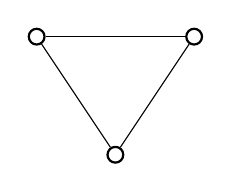
\begin{tikzpicture}[
        mass/.style = {draw,circle, minimum size=0.2cm, inner sep=0pt, thick},
        spring/.style = {decorate,decoration={zigzag, pre length=1cm,post length=1cm,segment length=5pt}},]
        \node[mass] (m1) at (1,1.5) {};
        \node[mass] (m2) at (-1,1.5) {};
        \node[mass] (m3) at (0,0) {};

        \draw (m1) -- (m2);
        \draw (m1) -- (m3);
        \draw (m2) -- (m3);
    \end{tikzpicture}
    \caption{A simple graph with three vertices and three edges}
\end{figure}
\begin{MyExercise}
    \textbf{
    Show that any finite-dimensional faithful representation $H$ of a matrix
    algebra $A$ is completely reducible. To do that show that the complement
    $W^{\perp}$ of an $A$-submodule $W\subset H$ is also an $A$-submodule
    of $H$.
}\newline

    $A\simeq \bigoplus_{i=1}^N M_{n_i}(\mathbb{C})$ is the matrix algebra
    then $H$ is a Hilbert $A$-bimodule and $W$ a submodule of $A$.
    Because we have $H = W \cup W^{\perp}$, then $W^{\perp}$ is naturally a
    $A$-submodule, because elements in $W^{\perp}$ need to satisfy the
    bimodularity.
\end{MyExercise}
\begin{definition}
    A $\Lambda$-decorated graph is given by an ordered pair $(\Gamma,
    \Lambda)$ of a finite graph $\Gamma$ and a set of positive integers
    $\Lambda$ with the labeling
    \begin{itemize}
        \item of the vetices $v\in \Gamma ^{(0)}$ given by $n(\nu) \in
            \Lambda$
        \item of the edges $e = (\nu _1, \nu _2) \in \Gamma ^{(1)}$ by
            operators
            \begin{itemize}
                \item $D_e: \mathbb{C}^{n(\nu _1)} \rightarrow
                    \mathbb{C}^{n(\nu _2)}$
                \item and $D_e^*: \mathbb{C}^{n(\nu _2)} \rightarrow
                    \mathbb{C}^{n(\nu _1)}$ its conjugate traspose
                    (pullback?)
            \end{itemize}
    \end{itemize}
    such that
    \begin{equation}
        n(\Gamma ^{(0)}) = \Lambda
    \end{equation}
\end{definition}
\begin{question}
    Would then $D_e$ be the pullback?
\end{question}
\begin{question}
    These graphs are important in the next chapter I should look
    into it more, I don't understand much here, specific
    how to construct them with the abstraction of a spectral triple...
\end{question}

The operator $D_e$ between $\textbf{n}_i$ and $\textbf{n}_j$ add up to
$D_{ij}$
\begin{align}
    D_{ij} = \sum\limits_{\substack{e = (\nu _1, \nu _2) \\ n(\nu _1) =
    \textbf{n}_i \\ n(\nu _2) = \textbf{n}_j}} D_e
\end{align}

\begin{theorem}
    There is a on to one correspondence between finite spectral triples
    modulo unitary equivalence and $\Lambda$-decorated graphs, given by
    associating a finite spectral triples $(A, H, D)$ to  a $\Lambda$ decorated
    graph $(\Gamma, \Lambda)$ in the following way:
    \begin{equation}
        A = \bigoplus _{n\in \Lambda} M_n(\mathbb{C}); \;\;\;
        H = \bigoplus _{\nu \in \Gamma ^{(0)}} \mathbb{C}^{n(\nu)}; \;\;\;
        D = \sum _{e \in \Gamma ^{(1)}} D_e + D_e^*
    \end{equation}
\end{theorem}
    \begin{figure}[h!]
    \centering
    \begin{tikzpicture}[
        mass/.style = {draw,circle, minimum size=0.3cm, inner sep=0pt, thick},
    ]

    \node[mass, label={\textbf{n}}] (m1) at (1,0) {};
    \draw (m1) to [out=330, in=210, looseness=25] node[above] {$D_e$} (m1);
    \end{tikzpicture}
    \caption{A $\Lambda$-decorated Graph of $(M_n(\mathbb{C}), \mathbb{C}^n,
    D = D_e + D_e^*)$}
\end{figure}

\begin{MyExercise}
    \textbf{
    Draw a $\Lambda$ decorated graph corresponding to the spectral triple
    $(A=\mathbb{C}^3, H=\mathbb{C}^3, D=\begin{pmatrix}0 & \lambda & 0\\
    \bar{\lambda} &0 &0 \\ 0&0&0\end{pmatrix})$
}\newline

\centering

\begin{tikzpicture}[
        mass/.style = {draw,circle, minimum size=0.4cm, inner sep=0pt, thick},
        spring/.style = {decorate,decoration={zigzag, pre length=1cm,post length=1cm,segment length=5pt}},]
        \node[mass] (m1) at (-1,1.5) {\textbf{1}};
        \node[mass] (m2) at (1,1.5) {\textbf{2}};
        \node[mass] (m3) at (3,1.5) {\textbf{3}};

        \draw[style=thick, -] (1.1,1.7) -- (-1.1,1.7);
        \draw[style=thick, -] (1.1,1.3) -- (-1.1,1.3);
    \end{tikzpicture}
    %    \captionof{figure}{Solution}
\end{MyExercise}
\begin{MyExercise}
    \textbf{
    Use $\Lambda$-decorated graphs to classify all finite spectral triples
    (modulo unitary equivalence) on the matrix algebra
    $A=\mathbb{C}\oplus M_2(\mathbb{C})$
}\newline

    \centering
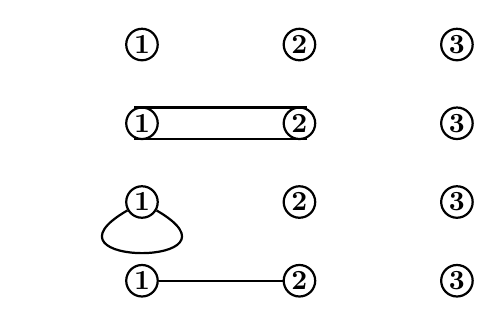
\begin{tikzpicture}[
        mass/.style = {draw,circle, minimum size=0.4cm, inner sep=0pt, thick},
        spring/.style = {decorate,decoration={zigzag, pre length=1cm,post length=1cm,segment length=5pt}},]
        \node[mass] (m1) at (-1,1) {\textbf{1}};
        \node[mass] (m2) at (1,1) {\textbf{2}};
        \node[mass] (m3) at (3,1) {\textbf{3}};

        \node[mass] (m4) at (-1,0) {\textbf{1}};
        \node[mass] (m5) at (1,0) {\textbf{2}};
        \node[mass] (m6) at (3,0) {\textbf{3}};

        \node[mass] (m7) at (-1,-1) {\textbf{1}};
        \node[mass] (m8) at (1,-1) {\textbf{2}};
        \node[mass] (m9) at (3,-1) {\textbf{3}};

        \node[mass] (m10) at (-1,-2) {\textbf{1}};
        \node[mass] (m11) at (1,-2) {\textbf{2}};
        \node[mass] (m12) at (3,-2) {\textbf{3}};

        \draw[style=thick, -] (1.1,0.2) -- (-1.1,0.2);
        \draw[style=thick, -] (1.1,-0.2) -- (-1.1,-0.2);
        \draw[style=thick, -] (m7) to [out=330, in=210, looseness=10] node[above] {} (m7);
        \draw[style=thick, -] (m10) -- (m11) ;

\end{tikzpicture}
%    \captionof{figure}{Solution $A=M_3(\mathbb{C})$}
\end{MyExercise}
\subsubsection{Graph Construction of Finite Spectral Triples}
\textbf{Algebra:}We know if a acts on a finite dimensional Hilbert space then
this C* algebra is isomorphic to a matrix algebra so $A \simeq
\bigoplus_{i=1}^{N}M_{n_i}(\mathbb{C})$. Where $i\in
\hat{A}$ represents an equivalence class and runs from $1$ to $N$,
thus $\hat{A}\simeq\{1,\dots, N\}$. We label equivalence classes by
$\textbf{n}_i$, then $\hat{A}\simeq\{\textbf{n}_1,\dots,\textbf{n}_N\}$.
\newline

\textbf{Hilbert Space:} Since every Hilbert space that acts faithfully on a
C* algebra is completely reducible, it is isomorphic to the composition
of irreducible representations. $H \simeq \bigoplus_{i=1}^N\mathbb{C}^{n_i}
\otimes V_i$. Where all $V_i$'s are Vector spaces, their dimension is the
multiplicity of the representation landed by $\textbf{n}_i$ to $V_i$ itself
by the multiplicity space.
\newline

\textbf{Finite Dirac Operator:} $D_{ij}$ is connecting nodes $\textbf{n}_i$
and $\textbf{n}_j$, with a symmetric map $D_{ij}:\mathbb{C}^{n_i}\otimes V_i
\rightarrow \mathbb{C}^{n_j}\otimes V_j$
\newline

To draw a graph, draw nodes in position $\textbf{n}_i\in \hat{A}$.
Multiple nodes at the same position represent multiplicities in $H$.
Draw lines between nodes to represent $D_{ij}$.

\begin{figure}[h!]
    \centering
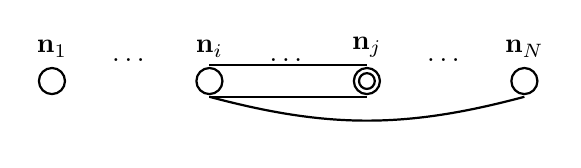
\begin{tikzpicture}
    \node[draw, label=above:{$\textbf{n}_1$},circle, thick] at (-3,0) {};
    \node[label=above:{$\dots$}] at (-2,0) {};
    \node[draw, label=above:{$\textbf{n}_i$},circle, thick] at (-1,0) {};
    \node[label=above:{$\dots$}] at (0,0) {};
    \node[draw, label=above:{$\textbf{n}_j$},circle, thick] at (1,0) {};
    \node[draw, label=above:{},circle, thick, inner sep=0cm, minimum
    size=0.2cm]  at (1,0) {};
    \node[label=above:{$\dots$}] at (2,0) {};
    \node[draw, label=above:{$\textbf{n}_N$},circle, thick] at (3,0) {};

        \draw[style=thick, -] (-1,-0.2) -- (1,-0.2);
        \draw[style=thick, -] (-1,0.2) -- (1,0.2);
        \path[style=thick, -] (-1,-0.2) edge[bend right=15]
        node[pos=0.5,below] {} (3,-0.2);
    \end{tikzpicture}
    \caption{Example}
\end{figure}


\end{document}
